\chapter{Présentation générale du CEA}
\pagenumbering{arabic}

\section{Le CEA}
\subsection{Généralités}
Le CEA (Commissariat à l’\' Energie Atomique et aux \' Energies Alternatives) est un établissement public industriel et commercial (EPIC) de droit privé. Ce statut lui permet d’avoir des activités avec différentes sociétés privées ou publiques tout en étant financé par l’état français. 
Le CEA a été créé en 1945 par l’ordonnance du général Charles De Gaulle. Il a pour but de réaliser les recherches sur le nucléaire et d'acquérir la maîtrise de l'atome. Il intervient ainsi dans quatre grands domaines de recherche : la défense, les énergies décarbonées, les technologies pour l’information et la santé, et la recherche fondamentale.
Il existe neuf centres de recherche CEA répartis sur le territoire français (Fig :\ref{centre_CEA}) (le centre Paris-Saclay comprend les sites de Saclay et de Fontenay aux Roses). Certains de ces centres sont liés aux applications militaires et sont contrôlés par la DAM (Direction des Applications Militaires) et d’autres sont liés aux applications civiles. Six PRTT (Plates-Formes Régionales de Transfert Technologique – (Hauts de France-Lille ; Grand Est-Metz ; Provence-Alpes-Côte d’Azur-Cadarache Gardane ; Occitanie-Pyrénées Méditerranée-Toulouse ; Nouvelle-Aquitaine-Bordeaux ; Pays de la Loire-Nates) appartenant au Pôle Recherche Technologique du CEA (CEA Tech) ont été créées en région, elles se rajoutent aux deux « bases arrières » historiques du CEA Tech de Saclay et de Grenoble. 




%\newpage
\subsection{Les directions opérationnelles du CEA}


Ces neuf centres se divisent au sein de quatre directions qui se partagent les grands domaines de compétence du CEA (\textit{cf}. Fig.~\ref{centre_CEA}):

\textbf{La DEN} : Direction de l’Energie Nucléaire qui opère sur les systèmes nucléaires du futur, l’optimisation du nucléaire industriel et sur le développement et l’exploitation d’outils expérimentaux et de simulation.

\textbf{La DRT }: Direction de la Recherche Technologique, qui se concentre sur les micro et nanotechnologies, les nouvelles technologies de l’énergie et les nanomatériaux ainsi que sur les systèmes numériques intelligents.

\textbf{La DRF }: Direction de la Recherche Fondamentale qui réalise la recherche des effets et applications du nucléaire au médical (radiothérapie, marquage biomoléculaire, etc.) et qui effectue la recherche traitant des sciences de la matière.

\textbf{La DAM} : Direction des Applications Militaires qui est le pôle Défense et Sécurité du CEA. La DAM travaille sur les armes nucléaires, la propulsion nucléaire, la sécurité et la non-prolifération ainsi que sur la défense conventionnelle.


\begin{figure}[h]
\centering
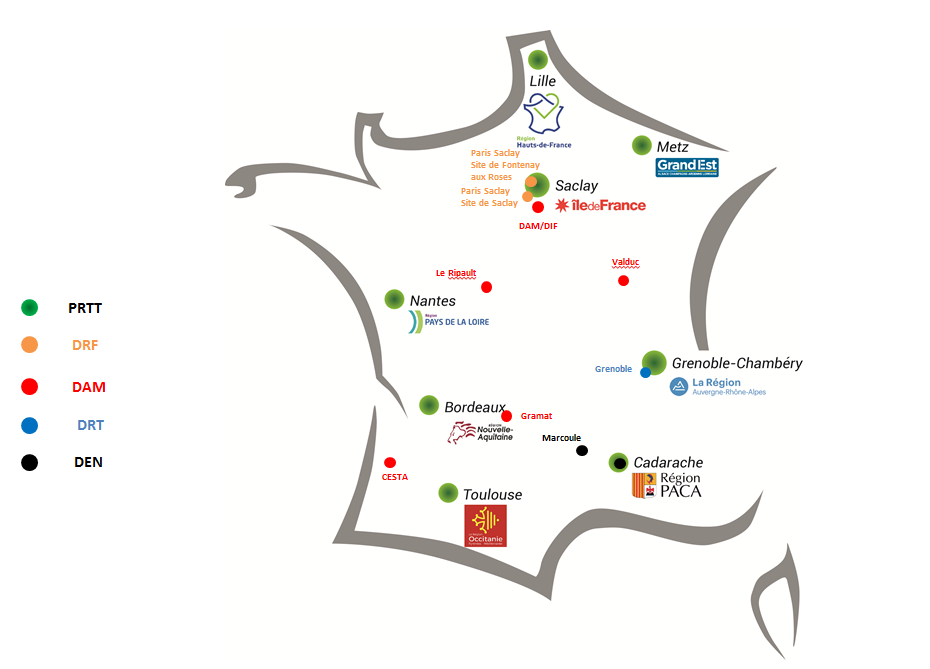
\includegraphics[scale=0.7]{fichier_configuration/carte_centres2018.png} 
\caption{Les centres CEA}
\label{centre_CEA}
\end{figure}
\FloatBarrier
\subsection{Le CEA en chiffres}

Le CEA était constitué, en 2017, de 33 laboratoires d'excellence, 27 équipes d’excellence et 3 initiatives d’excellence où travaillent 19 738 personnes (techniciens, ingénieurs, chercheurs et collaborateurs) soient 15 942 CDI, 1 183 doctorants, 160 post-doctorants, 554 alternants, 1 037 CDD et 862 autres salariées. Cela représente 5 milliards d’euros de budget (\SI{1.8}{\giga\euro} pour les activités défense, \SI{2.4}{\giga\euro} pour les activités civiles et \SI{0.8}{\giga\euro} pour les opérations assainissement et démantèlement), plus de 424 projets européens et 687 brevets en 2017 auprès de l’INPI (Institut National de la Propriété Industrielle) (4\textsuperscript{éme} place au niveau français derrière les industriels  Valéo, PSA et Safran et 1\textsuperscript{ère} place au niveau de organismes de recherche français).

\section{Le CEA/Gramat}

\subsection{Histoire du centre}

C’est en 1946 que le site de Gramat, situé au sein du parc naturel régional des causses du Quercy dans le Lot, est retenu pour implanter, dans le gouffre de Bèdes, des bancs d’essais de propulseurs de grande puissance (V2).

En 1956, le site devient le polygone d’expérimentations de la section atomique de la DEFA (Direction des Études et Fabrication d’Armement) et accueille les premiers essais liés au fonctionnement détonique des armes nucléaires.

En 1959, le site devient le CEG (Centre d’Etudes de Gramat), dépendant de la DGA (Délégation Générale pour l’Armement), puis, en 1965, les essais liés au fonctionnement détonique (non nucléaire) de l’arme nucléaire sont lancé. En 1965, des essais sur la dynamique des roches et les études de durcissement électromagnétique et mécanique sont mis en place.

C’est en janvier 2010 que le CEG de la DGA a rejoint le CEA. Il devient ainsi le dixième centre du CEA et le cinquième centre de la DAM.
Le site s’étend aujourd’hui sur 325 hectares et emploie 260 salariés ainsi que des stagiaires, apprentis et thésards. Il est le centre de référence pour l’étude de l’efficacité des armements et de la vulnérabilité des systèmes aux effets des armes conventionnelles et nucléaires.


\subsection{Domaine d'activité}

Les activités du CEA/Gramat se concentrent autour de trois domaines :
\begin{itemize}
\item{le nucléaire de défense (50~\%),}
\item{la défense conventionnelle (45~\%),}
\item{la sécurité globale (5~\%).}
\end{itemize}

Dans chacun de ces cas, le centre est spécialisé dans l’étude de la vulnérabilité des armes et systèmes de défense.

Le nucléaire de défense vise à étudier les effets du rayonnement, du souffle, du flash thermique et des ondes électromagnétiques générés par une arme.
Les recherches en défense conventionnelle permettent le développement des compétences en physique des explosifs, détonique, balistique terminale et en vulnérabilité des structures. La sécurité globale permet de mettre au profit de pouvoirs publics et de la sécurité des infrastructures, les compétences développées sur les deux points précédents. 

Enfin, la sécurité globale a pour objectif d’étudier la sécurité des infrastructures civiles ou militaires face aux actes malveillants, aux accidents ou aux catastrophes naturelles.

\subsection{Organisation de l'entreprise}

Le DEA (Département Effets des Armes) constitue l'organe principal de production technique du centre et est divisé en différents services, lesquels sont sous divisés en différents laboratoires (cf \textit{cf} Fig.~\ref{orga}). 

\begin{figure}[h]
\centering
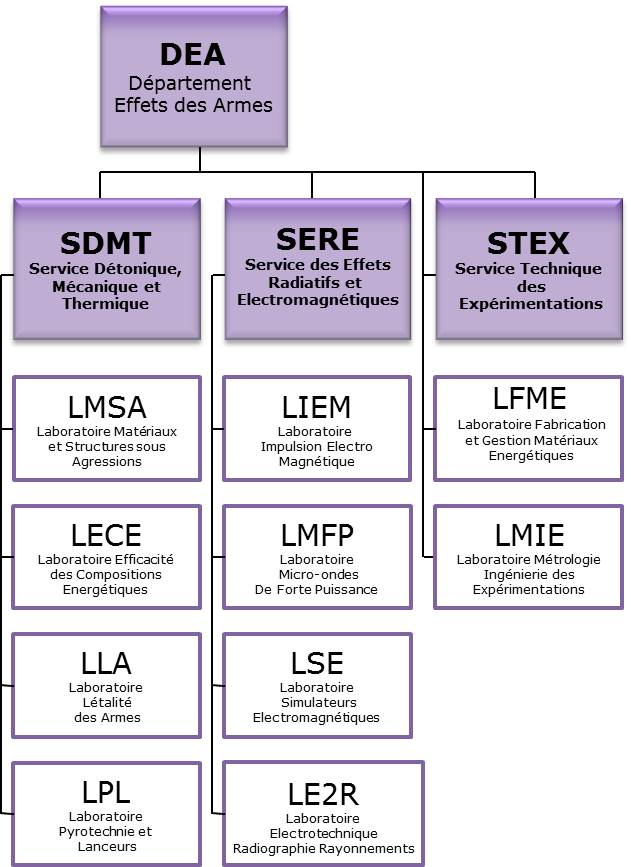
\includegraphics[scale=0.6]{fichier_configuration/organigramme.png} 
\caption{Organigramme du DEA du CEA/Gramat.}
\label{orga}
\end{figure}

\section{Positionnement dans l'entreprise}
\subsection{Besoins en logiciels du LECE}
Mon alternance se déroulera au Service Détonique, Mécanique et Thermique (SDMT) dans le Laboratoire  Efficacité des Compositions Énergétiques (LECE). Ce service travaille principalement sur l'effet des armes conventionnelles et les moyens de s'en protéger. Environ 70 personnes travaillent au SDMT, principalement des chercheurs et techniciens. La quinzaine de membres du LECE s'intéressent, eux, principalement à la modélisation et aux effets des explosifs. Dans le cadre de leur travaux, les chercheurs peuvent être amenés à développer des logiciels répondant à des besoins assez spécifiques.

C'est dans ce contexte que j'interviens au LECE. Plusieurs codes propres au laboratoire pourraient être améliorés. Les personnes travaillant sur ces codes sont principalement des ingénieurs chercheurs et n'ont pas forcément le temps et les compétences de s'occuper de la partie plus \og informatique \fg{} du logiciel.  

\subsection{Outils mis à disposition}
Pour des raisons de sécurité et de confidentialité, l'intégralité du matériel informatique mis à disposition est la propriété du CEA et il n'est pas possible d'utiliser du matériel personnel (PC, clef USB\dots{}). Il est aussi à noter que mon poste de travail est totalement déconnecté d'Internet. Il est donc très complexe d' installer des logiciels \og extérieurs \fg. Fort heureusement le centre fournit des services et logiciels suffisant pour que je puisse travailler dans de bonnes conditions : 
\begin{itemize}
\item un poste fixe sous Windows;
\item un accès à toutes les ressources du réseau interne (stockage distant, intranet, mail interne...);
\item le pack Office, TexMaker et d'autres outils \og bureautique \fg;
\item python 2.7 32~bits et Python 3.3 64~bits avec l'IDE Spyder;
\item des compilateurs C, C++ et Fortran 64~bits pour Windows et Linux;
\item un accès SSH à des machines Linux;
\item un serveur Git (GitLab) interne au CEA Gramat;
\item un serveur SQL (MySQL) lui aussi interne au CEA Gramat;
\item un accès à des postes reliés à internet pour rechercher des informations.
\end{itemize}
Les outils mis à ma disposition sont suffisants pour remplir ma première mission et sans doute les suivantes. 
 	